\begin{titre}[Représentation et utilisation des solides]

\Titre{Utiliser les solides}{2,5}
\end{titre}

\impress{1}{
\begin{CpsCol}
\textbf{Développer sa vision de l'espace}
\begin{description}
\item[$\square$] Connaître la définition des solides
\item[$\square$] Utiliser des solides concrets pour illustrer certaines propriétés de géométrie
\item[$\square$] Calculer des grandeurs (aires, volumes)
\end{description}
\end{CpsCol}
}


\Rec{1}{RepS-30}

\impress{1}{
\begin{PpT}{Volumes des prismes droits et pyramides; cylindres et cônes}
 
\begin{enumerate}
\begin{multicols}{2}
 \item Pavé droit (ou parallélépipède rectangle):\\
$V=largeur \times longueur \times hauteur$
\begin{center}
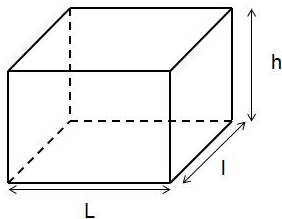
\includegraphics[scale=0.4]{RepS-pave_droit.png} 
\end{center} 


\item Prisme droit:\\  $V=A_{base} \times hauteur$

\begin{center}
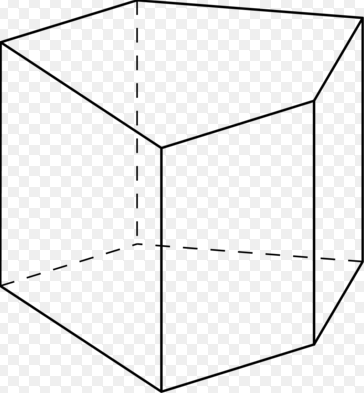
\includegraphics[scale=0.2]{RepS-prisme_droit.png} 
\end{center}


\item  Cylindre:\\ 
$V=A_{base} \times hauteur = \pi R^2 \times hauteur$

\begin{center}
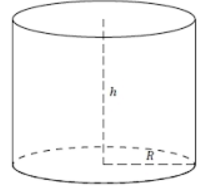
\includegraphics[scale=0.4]{RepS-cylindre.png} 
\end{center}


\item Pyramide:\\ $V= \frac{ A_{base} \times hauteur}{3}$

\begin{center}
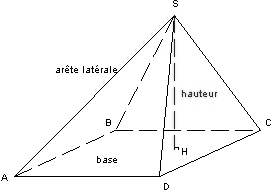
\includegraphics[scale=0.5]{RepS-pyramide.png} 
\end{center}

\item Cône de révolution:\\
$V=\frac{ A_{base} \times hauteur}{3}=\frac{ \pi \times R^2 \times hauteur}{3}$

\begin{center}
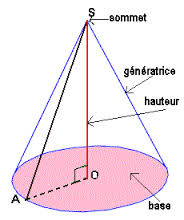
\includegraphics[scale=0.3]{RepS-cone.png} 
\end{center}
\end{multicols}
\end{enumerate}

\end{PpT}

\begin{PpT}{Aire d'une sphère;volume d'une boule}

L´aire de la sphère est donné par: $A=4 \pi R^2$\\
Le volume d´une boule est donné par: $V=\frac{4}{3} \pi R^3$
\begin{center}
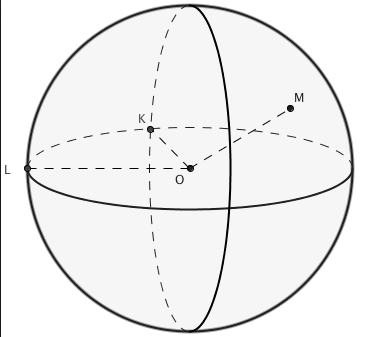
\includegraphics[scale=0.4]{RepS-Sphere.jpg} 
\end{center}
\end{PpT}
}

\mini{
\AD{1}{RepS-59}

\Exo{1}{RepS-35}
}{
\Exo{1}{RepS-38}

\Exo{1}{RepS-44}
}

\impress{1}{
\ \\
\vspace{0.2cm}
}

\Exo{1}{RepS-49}

\Exo{1}{RepS-43}

\mini{
\Exo{1}{RepS-46}
}{
\Exo{1}{RepS-47}
}

\Exo{1}{RepS-50}

\impress{0}{

\vspace{2cm}


{\Large {\color{violet}Aucun exercice sur ce chapitre dans le cahier}}


\begin{autoeval}
\begin{tabular}{p{12cm}p{0.5cm}p{0.5cm}p{0.5cm}p{1cm}}
\textbf{Compétences visées} &  M I & MF & MS  & TBM \vcomp \\ 
Connaître la définition des solides & $\square$ & $\square$  & $\square$ & $\square$ \vcomp \\
Utiliser des solides concrets pour illustrer certaines propriétés & $\square$ & $\square$  & $\square$ & $\square$ \vcomp \\
Calculer des grandeurs (aires, volumes) & $\square$ & $\square$  & $\square$ & $\square$ \vcomp \\
\end{tabular}
{\footnotesize MI : maitrise insuffisante ; MF = Maitrise fragile ; MS = Maitrise satisfaisante ; TBM = Très bonne maitrise}
\end{autoeval}
}